%label:"exr:heegaardFloerLensSpace"
%type:"exercise"
%name:"Heegaard Floer cohomology of lens spaces"


        A \emph{Lens space} $L(p,q)$ can be defined as the $3$-manifold with a Heegaard splitting of genus 1, with an $\alpha$-curve given by a longitude of the the torus, and the $\beta$-curve in the class $(p, q)$. Use the above obstruction to compute $\widehat{HHF}^\bullet(L(p,q))$.
        %label:"fig:heegaardDiagramLensSpace"
%type:"figure"
%author:JeffHicks
%name:"Heegaard diagram for the Lens space $L(2,3)"
%caption:"The Heegaard diagram for the Lens space $L(2,3)$"

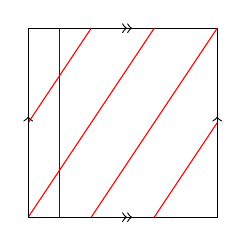
\begin{tikzpicture}[scale=2]

    \draw  (2.2,2.4) rectangle (3.4,1.2);
    \draw[blue] (2.4,2.4) -- (2.4,1.2);
    \draw[red] (2.2,1.2) -- (3,2.4) (3,1.2) -- (3.4,1.8) (2.2,1.8) -- (2.6,2.4) (2.6,1.2) -- (3.4,2.4);
    \draw[->] (2.2,1.2) -- (2.2,1.84);
\draw[->] (3.4,1.2) -- (3.4,1.84);
\draw[->>] (2.6,1.2) -- (2.86,1.2);
\draw[->>] (2.6,2.4) -- (2.86,2.4);
\end{tikzpicture}
    

